\section{top}
\label{chap:linux_top}

top

显示Linux进程

top提供了运行系统的动态实时视图。它可以显示系统摘要信息以及当前由Linux内核管理的进程或线程的列表。所显示的系统摘要信息的类型以及为流程显示的信息的类型、顺序和大小都是用户可配置的
该配置可以在重启时保持不变。

交互式命令

\menlo{l}     切换是否显示系统平均负载

\menlo{c}     切换程序名或命令行的显示

\menlo{d}     修改屏幕刷新时间

\menlo{i}     切换显示所以线程或任务

\menlo{H}     切换为线程模式

\menlo{t}     切换Task/Cpu显示状态

\menlo{m}     切换内存模式显示状态


OPTIONS

-b  \par
\qquad 批处理模式操作,可用于将top输出内容发送到其他程序或者文件中

-c \par 
\qquad 显示完整命令行或者程序名

-d :Delay-time interval as:  -d ss.t (secs.tenths)  \par 
\qquad  指定屏幕更新时间间隔;也可以使用交互命令d或者s。可以填写分数秒。

-H  :Threads-mode operation \par
\qquad  指定显示各个线程,如果没有此选项,则显示每个进程中所有线程的总和。也可以使用交互命令H。

-i  :Idle-process toggle    \par 
\qquad 使top不显示任何闲置或者僵死进程。

-n  :Number-of-iterations limit as:  -n number  \par 
\qquad  循环显示的次数

-o  :Override-sort-field as:  -o fieldname  \par
\qquad 指定将对那些任务字段进行排序。可以在字段名前加上+或者-用来覆盖排序方向。前置+将强制从高到低排序,而-是从低到高排序。可用字段名可以参选下面的-O选项。

-O  :Output-field-names \par
\qquad 打印可用的字段名

-p  :Monitor-PIDs mode as:  -pN1 -pN2 ...  or  -pN1,N2,N3 ...\par
\qquad 仅监视具有指定进程id的进程。此选项最多可以使用20次,或者您可以提供最多20个pid的逗号分隔列表。如果需要恢复,可以使用=,u或U。

-S  :Cumulative-time toggle \par
\qquad 当启用累积时间模式时,每个进程都会列出它和它死去的子进程所使用的cpu时间。

-u | -U  :User-filter-mode as:  -u | -U number or name\par 
\qquad 只显示与给定的用户id或用户名匹配的进程。-u选项匹配有效用户,而-U选项匹配任何用户(实际的、有效的、已保存的或文件系统)。在用户id或名称前面加上感叹号('!'),指示top只显示与提供的用户不匹配的进程。


输出内容解释

\begin{figure}[H]
    \centering
    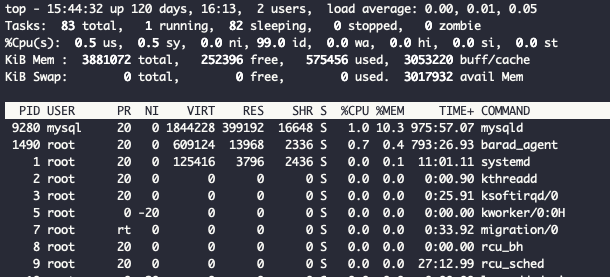
\includegraphics[width=1\textwidth]{linux/top-1.png}
    \caption{top}
\end{figure}



第一行输出任务为UPTIME and LOAD Averages

\begin{lstlisting}[language=cshell]

#   top - 15:52:24 up 120 days, 16:21,  2 users,  load average: 0.14, 0.10, 0.07

\end{lstlisting}

第二行为任务(进程)或者线程信息;进程或者线程的切换可以通过交互命令H。 分为:运行;休眠;停止;僵尸

\begin{lstlisting}[language=cshell]

#   Tasks:  86 total,   1 running,  85 sleeping,   0 stopped,   0 zombie

#   Threads: 149 total,   1 running, 148 sleeping,   0 stopped,   0 zombie

\end{lstlisting}


第三行为CPU状态信息


\begin{lstlisting}[language=cshell]

#   %Cpu(s):  0.7 us,  0.7 sy,  0.0 ni, 98.7 id,  0.0 wa,  0.0 hi,  0.0 si,  0.0 st
#              a   b      c  d 
#   %Cpu(s):  0.3/0.5     1[|

\end{lstlisting}

us, user    : 用户空间占用CPU百分比(time running un-niced user processes)    \par
sy, system  : 内核空间占用CPU百分比(time running kernel processes)  \par
ni, nice    : 用户进程空间内改变过优先级的进程占用CPU百分比(time running niced user processes)   \par
id, idle    : 空闲CPU百分比(time spent in the kernel idle handler)  \par
wa, IO-wait : 等待输入输出的CPU时间百分比(time waiting for I/O completion)       \par
hi : 硬中断(Hardware IRQ)占用CPU的百分比(time spent servicing hardware interrupts)      \par
si : 软中断(Software Interrupts)占用CPU的百分比(time spent servicing software interrupts)      \par
st : hypervisor vm占用的CPU时间的百分比(time stolen from this vm by the hypervisor) \par

在使用交互命令t切换到cpu状态模式时,还会额外显示一行CPU摘要信息,如上面展示第二行

a) 是 us 和 ni 之和 \par
b) 是 sy 百分比 \par
c) 是总和   \par
d) 是可视化图像 \par


内存使用情况

默认情况下,第1行反映物理内存,分类为:\par
total(物理内存总量), free(空闲内存总量), used(使用的物理内存总量) and buff/cache(用作内核缓存的内存量)

第2行反映的主要是虚拟内存,分为以下几类:\par
total(交换区总量), free(闲交换区总量), used(使用的交换区总量) and avail(可用物理内存)

此行的avail 指启动新应用程序时可用的物理内存的估计值不包含swapping。与free命令不同的是,free试图分析易于回收的页面缓存和内存片。

可以通过交互命令E切换单位

\begin{lstlisting}[language=cshell]

# MiB Mem :   3790.1 total,    228.7 free,    568.1 used,   2993.2 buff/cache
# MiB Swap:      0.0 total,      0.0 free,      0.0 used.   2941.0 avail Mem

\end{lstlisting}

在内存模式(使用交互命令m)下,会显示两行简短的简要:

\begin{lstlisting}[language=cshell]

            a    b          c
MiB Mem : 23.2/3790.1   [|||||                         ]
MiB Swap:  0.0/0.0      [                              ]

\end{lstlisting}

a) 使用百分比

b) 总物理内存

c) 图形化展示


\begin{lstlisting}[language=cshell]

PID USER      PR  NI    VIRT    RES    SHR S  %CPU %MEM     TIME+ COMMAND
9280 mysql     20   0 1844228 399192  16648 S   0.7 10.3 990:08.75 mysqld
1490 root      20   0  609124  13968   2336 S   0.3  0.4 803:34.96 barad_agent

\end{lstlisting}


列含义



1. \%CPU  -- CPU使用率  \par
\qquad CPU使用时间占比

2. \%MEM  --  内存使用 (常驻内存)   \par
\qquad 进程使用的物理内存百分比

3. CGROUPS  --  Control Groups  \par
The names of the control group(s) to which a process belongs, or `-' if not applicable for that process.

Control Groups provide for allocating resources (cpu, memory, network bandwidth, etc.) among installation-defined groups of processes.  They enable fine-grained control over allocating, denying, prioritizing, managing and monitoring those resources.

Many different hierarchies of cgroups can exist simultaneously on a system and each hierarchy is attached to one or more subsystems.  A subsystem represents a single resource.

Note:  The CGROUPS field, unlike most columns, is not fixed-width.  When displayed, it plus any other variable width columns will be allocated all remaining screen width (up to the maximum 512 characters).  Even so, such variable width fields could still
suffer truncation.  See topic 5c. SCROLLING a Window for additional information on accessing any truncated data.

4. CODE  --  Code Size (KiB) \par
\qquad 可执行代码占用物理内存大小,也称为文本常驻集(Text Resident Set)大小或TRS。

5. COMMAND  --  Command Name or Command Line    \par
Display the command line used to start a task or the name of the associated program.  You toggle between command line and name with `c', which is both a command-line option and an interactive command.

When you've chosen to display command lines, processes without a command line (like kernel threads) will be shown with only the program name in brackets, as in this example:
    [kthreadd]

This field may also be impacted by the forest view display mode.  See the `V' interactive command for additional information regarding that mode.

Note: The COMMAND field, unlike most columns, is not fixed-width.  When displayed, it plus any other variable width columns will be allocated all remaining screen width (up to the maximum 512 characters).  Even so, such variable width fields could  still
suffer truncation.  This is especially true for this field when command lines are being displayed (the `c' interactive command.)  See topic 5c. SCROLLING a Window for additional information on accessing any truncated data.


6. DATA  --  Data + Stack Size (KiB)    \par
The amount of physical memory devoted to other than executable code, also known as the Data Resident Set size or DRS.

7. ENVIRON  --  Environment variables   \par
Display all of the environment variables, if any, as seen by the respective processes.  These variables will be displayed in their raw native order, not the sorted order you are accustomed to seeing with an unqualified `set'.

Note:  The ENVIRON field, unlike most columns, is not fixed-width.  When displayed, it plus any other variable width columns will be allocated all remaining screen width (up to the maximum 512 characters).  Even so, such variable width fields could still
suffer truncation.  This is especially true for this field.  See topic 5c. SCROLLING a Window for additional information on accessing any truncated data.

8. Flags  --  Task Flags    \par
This column represents the task's current scheduling flags which are expressed in hexadecimal notation and with zeros suppressed.  These flags are officially documented in <linux/sched.h>.

9. GID  --  有效组id \par

10. GROUP  --  有效组名 \par

11. NI  --  Nice Value  \par
The nice value of the task.  A negative nice value means higher priority, whereas a positive nice value means lower priority.  Zero in this field simply means priority will not be adjusted in determining a task's dispatch-ability.

12. P  --  Last used CPU (SMP)  \par
A number representing the last used processor.  In a true SMP environment this will likely change frequently since the kernel intentionally uses weak affinity.  Also, the very act of running top may break this weak affinity and cause  more  processes  to
change CPUs more often (because of the extra demand for cpu time).

13. PGRP  --  Process Group Id  \par
Every  process  is  member of a unique process group which is used for distribution of signals and by terminals to arbitrate requests for their input and output.  When a process is created (forked), it becomes a member of the process group of its parent.
By convention, this value equals the process ID (see PID) of the first member of a process group, called the process group leader.

14. PID  --  进程ID \par

15. PPID  --  父进程ID \par

16. PR  --  Priority    \par
The scheduling priority of the task.  If you see `rt' in this field, it means the task is running under real time scheduling priority.

Under linux, real time priority is somewhat misleading since traditionally the operating itself was not preemptible.  And while the 2.6 kernel can be made mostly preemptible, it is not always so.

17. RES  --  驻留内存大小 (KiB) \par
\qquad 线程在使用的非swap物理内存大小(The non-swapped physical memory a task is using.)


18. RUID  --  真实uid \par
The real user ID.

19. RUSER  --  真实用户名 \par

20. S  --  进程状态(Process Status) \par

    D = 不可中断睡眠状态(uninterruptible sleep)
    R = 运行状态(running)
    S = 睡眠状态(sleeping)
    T = stopped by job control signal
    t = stopped by debugger during trace
    Z = 僵尸状态(zombie)

Tasks shown as running should be more properly thought of as ready to run --  their task\_struct is simply represented on the Linux run-queue.  Even without a true SMP machine, you may see numerous tasks in this state depending on  top's  delay  interval
and nice value.

21. SHR  --  Shared Memory Size (KiB)   \par
The amount of shared memory available to a task, not all of which is typically resident.  It simply reflects memory that could be potentially shared with other processes.

22. SID  --  Session Id \par
A  session  is  a  collection  of  process groups (see PGRP), usually established by the login shell.  A newly forked process joins the session of its creator.  By convention, this value equals the process ID (see PID) of the first member of the session,
called the session leader, which is usually the login shell.

23. SUID  --  Saved User Id \par
The saved user ID.

24. SUPGIDS  --  Supplementary Group IDs    \par
The IDs of any supplementary group(s) established at login or inherited from a task's parent.  They are displayed in a comma delimited list.

Note: The SUPGIDS field, unlike most columns, is not fixed-width.  When displayed, it plus any other variable width columns will be allocated all remaining screen width (up to the maximum 512 characters).  Even so, such variable width fields could  still
suffer truncation.  See topic 5c. SCROLLING a Window for additional information on accessing any truncated data.

25. SUPGRPS  --  Supplementary Group Names  \par
The names of any supplementary group(s) established at login or inherited from a task's parent.  They are displayed in a comma delimited list.

Note:  The SUPGRPS field, unlike most columns, is not fixed-width.  When displayed, it plus any other variable width columns will be allocated all remaining screen width (up to the maximum 512 characters).  Even so, such variable width fields could still
suffer truncation.  See topic 5c. SCROLLING a Window for additional information on accessing any truncated data.

26. SUSER  --  Saved User Name  \par
The saved user name.

27. SWAP  --  Swapped Size (KiB)    \par
The non-resident portion of a task's address space.

28. TGID  --  线程组ID(Thread Group Id) \par
\qquad 任务所属的线程组的ID。它是线程组领导的PID。在内核术语中,它表示那些共享mm\_struct的任务。

29. TIME  --  CPU Time  \par
Total CPU time the task has used since it started.  When Cumulative mode is On, each process is listed with the cpu time that it and its dead children have used.  You toggle Cumulative mode with `S', which is both a command-line option and an interactive
command.  See the `S' interactive command for additional information regarding this mode.

30. TIME+  --  CPU Time, hundredths \par
The same as TIME, but reflecting more granularity through hundredths of a second.

31. TPGID  --  Tty Process Group Id \par
The process group ID of the foreground process for the connected tty, or -1 if a process is not connected to a terminal.  By convention, this value equals the process ID (see PID) of the process group leader (see PGRP).

32. TTY  --  Controlling Tty    \par
The  name  of  the controlling terminal.  This is usually the device (serial port, pty, etc.) from which the process was started, and which it uses for input or output.  However, a task need not be associated with a terminal, in which case you'll see `?'
displayed.

33. UID  --  用户ID;进程所有者的真实用户ID   \par

34. USED  --  Memory in Use (KiB)   \par
This field represents the non-swapped physical memory a task has used (RES) plus the non-resident portion of its address space (SWAP).

35. USER  --  用户名;进程所有者的真实用户名  \par

36. VIRT  --  Virtual Memory Size (KiB) \par
The total amount of virtual memory used by the task.  It includes all code, data and shared libraries plus pages that have been swapped out and pages that have been mapped but not used.

37. WCHAN  --  Sleeping in Function \par
Depending on the availability of the kernel link map (System.map), this field will show the name or the address of the kernel function in which the task is currently sleeping.  Running tasks will display a dash ('-') in this column.

By displaying this field, top's own working set could be increased by over 700Kb, depending on the kernel version.  Should that occur, your only means of reducing that overhead will be to stop and restart top.

38. nDRT  --  Dirty Pages Count \par
The number of pages that have been modified since they were last written to auxiliary storage.  Dirty pages must be written to auxiliary storage before the corresponding physical memory location can be used for some other virtual page.

39. nMaj  --  Major Page Fault Count    \par
The number of major page faults that have occurred for a task.  A page fault occurs when a process attempts to read from or write to a virtual page that is not currently present in its address space.  A major page fault is when auxiliary  storage  access
is involved in making that page available.

40. nMin  --  Minor Page Fault count    \par
The number of minor page faults that have occurred for a task.  A page fault occurs when a process attempts to read from or write to a virtual page that is not currently present in its address space.  A minor page fault does not involve auxiliary storage
access in making that page available.

41. nTH  --  Number of Threads  \par
The number of threads associated with a process.

42. nsIPC  --  IPC namespace    \par
The Inode of the namespace used to isolate interprocess communication (IPC) resources such as System V IPC objects and POSIX message queues.

43. nsMNT  --  MNT namespace    \par
The Inode of the namespace used to isolate filesystem mount points thus offering different views of the filesystem hierarchy.

44. nsNET  --  NET namespace    \par
The Inode of the namespace used to isolate resources such as network devices, IP addresses, IP routing, port numbers, etc.

45. nsPID  --  PID namespace    \par
The Inode of the namespace used to isolate process ID numbers meaning they need not remain unique.  Thus, each such namespace could have its own `init' (PID \#1) to manage various initialization tasks and reap orphaned child processes.

46. nsUSER  --  USER namespace  \par
The Inode of the namespace used to isolate the user and group ID numbers.  Thus, a process could have a normal unprivileged user ID outside a user namespace while having a user ID of 0, with full root privileges, inside that namespace.

47. nsUTS  --  UTS namespace    \par
The Inode of the namespace used to isolate hostname and NIS domain name.  UTS simply means "UNIX Time-sharing System".

48. vMj  --  Major Page Fault Count Delta   \par
The number of major page faults that have occurred since the last update (see nMaj).

49. vMn  --  Minor Page Fault Count Delta   \par
The number of minor page faults that have occurred since the last update (see nMin).








